\section*{Problemas}

\begin{problema} \label{problema:3.1}
	Escribir los términos de cada una de las siguientes sumas:
	\begin{enumerate}
		\item $\displaystyle\sum_{j=0}^{6}X_{j}=$ 
		\item $\displaystyle\sum_{k=1}^{4}\left( Y_{k}-3 \right)^{2}=$ 
		\item $\displaystyle\sum_{k=1}^{N}a=$ 
		\item $\displaystyle\sum_{n=2}^{5}{f_{n}}X_{n}= $ 
		\item $\displaystyle\sum_{m=0}^{3}\left( X_{m}-a \right)=$
	\end{enumerate}
	%
	%
\end{problema}
%


\begin{problema}
	\label{problema:3.10}
	De 100 números, 20 fueron 4, 40 fueron 5, 30 fueron 6 y los restantes fueron 7. Encuentre su media aritmética.
\end{problema}




\begin{problema}
	\label{problema:3.13}
	Los pesos medio de cuatro grupos de estudiantes que constan de 15, 20, 10 y 18 individuos son 162, 148, 153 y 140 libras, respectivamente. Encuentre el peso medio de todos los estudiantes.
\end{problema}



%

\begin{problema}
	\label{problema:3.15}
	
	Usando la distribución de frecuencias de las estaturas que se presenta en la siguiente tabla, hallar la estatura media de 100 estudiantes de cierta universidad.
	\begin{figure}
		%%%%%%%%%%%%%%%%%%%%%%%%%%%%%%%%%%%%%%%%%%%%%%%%%%%%%%%%%%%%%%%%%%%%%%%%%%%%%%%%%%%%%%%
		%%% You will need to add \usepackage{wrapfig} to your preamble to use textwrapping %%%
		%%%%%%%%%%%%%%%%%%%%%%%%%%%%%%%%%%%%%%%%%%%%%%%%%%%%%%%%%%%%%%%%%%%%%%%%%%%%%%%%%%%%%%%
		\centering
		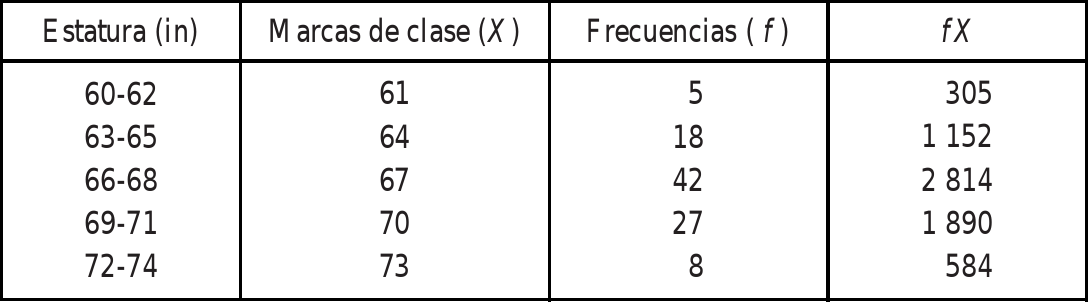
\includegraphics[width=10cm,keepaspectratio=true]{./images/tab0301.png}
		% tab0301.png: 0x0 pixel, 300dpi, 0.00x0.00 cm, bb=
		\label{tab:0301}
	\end{figure}
\end{problema}




\begin{problema}
	\label{problema:3.18}
	Si las desviaciones de $N$ números $X_{1},..,X_{N}$ respecto a un \emph{pivote} $P$ están dada por $d_{i}=X_{i}-P, \; i=1,...,N$ respectivamente, demostrar que
	\begin{align}
		\bar{X}=P+\dfrac{\sum d}{N}.
	\end{align}
\end{problema}



\begin{problema}
	\label{problema:3.16}
	Demostrar que la suma de las desviaciones $d_{1},d_{2},...,d_{N}$ de $X_{1},X_{2},...,X_{N}$ usando como pivote su media $\bar{X}$ es igual a cero.
\end{problema}



\begin{problema}
	\label{problema:3.17}
	Si $Z_{i}=X_{i}+Y_{i}, \; i=1,2,...,N,$ demostrar que $\bar{Z}=\bar{X}+\bar{Y}.$
\end{problema}




\begin{problema}
	\label{problema:3.19}
	Halle la media aritmética de los números 5,8,11,9,12,6,14 y 10 eligiendo como \emph{pivote} a) $P=9$ y b) $P=20.$
\end{problema}




\begin{problema}
	\label{problema:3.20}
	Utilice la marca de la clase media como pivote, para calcular la estatura de los estudiantes en la tabla \ref{tab:0301}.
\end{problema}



\begin{problema}
	\label{problema:3.28}
	Encontrar el peso mediano a partir de la siguiente tabla
	\begin{figure}[ht]
		\centering
		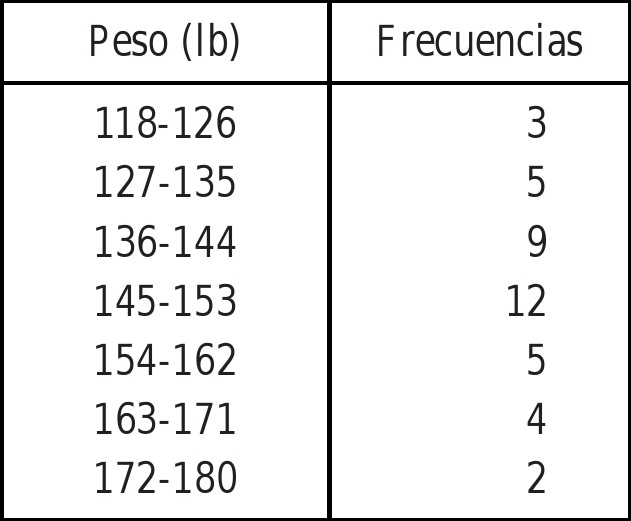
\includegraphics[height=5cm,keepaspectratio=true]{./images/tab0307.png}
		% tab0307.png: 0x0 pixel, 300dpi, 0.00x0.00 cm, bb=
		\label{tab:0307}
	\end{figure}
	
\end{problema}

